% This is meant to be a helpful template for papers being submitted to
% Medical Physics. It is not mandatory.
%
% Please send suggestions/improvements to drogers@physics.carleton.ca
% Sept 24, 2018
%

\documentclass[12pt,twoside]{article}   %For printing on two sides of page
					%It doesn't work with showkeys so
					%if using showkeys, use following
%\documentclass[12pt]{article}		%use with showkeys or to print one sided
\usepackage[super,sort,comma]{natbib}
%\usepackage[super,sort&compress,comma]{natbib}
% use the version without compress to get everything working. Then on ONE,
% and ONLY ONE FINAL RUN, use the version with compress to change 1,2,3,4
% to 1-4 etc in the citations.  Otherwise hyperref gets confused.


\usepackage{fancyhdr}		%Gives headers and footers defined below
\renewcommand{\footrulewidth}{0.4pt} %thickness of line above footer

\usepackage{showkeys}		%may use for drafting
				%comment out for final submission

%The following is useful for creating captions for figures and tables that have
%a different font and different width on the page. This separates them from
%text.
\newcommand{\captionv}[3]{\begin{center}\parbox{#1cm}{\caption[#2]{{\sf #3}}}
        \end{center}}
	%use as   \captionv{N}{B}{C}
	%first entry,N, is width of caption in cm
	%second entry, B, is a short title that appears in list of figure/tables
	%     B can be blank. The lists are not needed
	%third entry, C, is the caption for the figure or the table
	%    Note that the \label{fig_text} should be part of entry C.

\usepackage[section]{placeins}   %
%above package forces all floats (tables figures) to be processed before a
%new section starts. Unlike using \clearpage, this will start the section
%on the same page as the float, but after it.
%might not work with subsections, but if that is the case, put
%  \FloatBarrier just before the \subsection

\usepackage{graphicx}

%following lines fix up style of bibliography to be superscripts
\makeatletter \renewcommand\@biblabel[1]{$^{#1}$} \makeatother
 \setlength{\bibhang}{0em}
 \setlength{\labelsep}{1em}     
 \setlength{\itemindent}{-\bibhang}
 \setlength{\leftmargin}{\bibhang}


%set dimensions of the page for 8.5x11 inch paper
\setlength{\textwidth}{16.5cm}
\setlength{\headwidth}{16cm}		%for fancy page style only
\setlength{\textheight}{22.6cm} 
\setlength{\oddsidemargin}{-1mm}
\setlength{\evensidemargin}{-2mm} 
\setlength{\topmargin}{-1.0cm}

\setlength{\parindent}{2em}   %indent paragraph 2 letters m
\setlength{\parskip}{1.3ex}   %paragraph break
\setlength{\floatsep}{0pt}
\setlength{\textfloatsep}{0pt}		%space below a figure/table def 20pt
\setlength{\intextsep}{0pt}		%space below a figure/table def 20pt
					%p142 compendium

%Following is for Med Phys numbering  I.A.1  etc
\renewcommand{\thesection}{{\sf \Roman{section}}.}
\renewcommand{\thesubsection}{\thesection{\sf \Alph{subsection}}.}
\renewcommand{\thesubsubsection}{\thesubsection{\sf \arabic{subsubsection}}.}
\renewcommand{\theparagraph}{\alph{paragraph}.}


% following is useful during drafting when you want to flag something for
% other authors or for yourself. It can be used throughout the text.
\newcommand{\note}[1]{\mbox{}\\ \noindent \rule{16cm}{0.5mm} \\
{\em #1} \\ \noindent \rule{16cm}{0.5mm}
\typeout{    }
\typeout{***********note active on this page *************************}
\typeout{Note: #1  }
\typeout{****************************************end Note}
}

% Uncomment the following to remove all notes from the paper
% \renewcommand{\note}[1]{}


% These can be used to identify where a figure or table is first referenced 
% by placing a margin note.  If the figures/tables are inserted in the text
% they are not needed.

\newcommand{\mfig}[1]{\marginpar{{\sf Fig~\ref{#1} }}}
\newcommand{\mtab}[1]{\marginpar{{\sf Table~\ref{#1} }}}

%Following are just useful shortcuts and not mandatory
\newcommand{\cen}[1]{\begin{center} #1 \end{center}}
\newcommand{\eqn}[1]{\begin{equation} #1 \end{equation} }

%The following allow lists to be more compact than the default. Not
%mandatory, but useful.
\newenvironment{packed_enum}{
\begin{enumerate}
  \setlength{\itemsep}{1pt}
  \setlength{\parskip}{0pt}
  \setlength{\parsep}{0pt}
}{\end{enumerate}}

\newenvironment{packed_item}{
\begin{itemize}
  \setlength{\itemsep}{1pt}
  \setlength{\parskip}{0pt}
  \setlength{\parsep}{0pt}
}{\end{itemize}}

\renewcommand{\refname}{}       %

% The following only needed if you use the headers/footers. Not essential
% but can be useful      

% [on even pages]{on odd pages} %even pages only active f using twosided
				%if no even given, uses same for both
% lhead is left head, etc
\lhead[{\sffamily page~\thepage}]{{\sffamily  Temperature and time stability of a radiochromic dosimeter: Printed \today}}
% the $Date:$ below is replaced by the date the file was last edited when using
% CVS.  If not being used, comment this out.
\lfoot[{\sf \leftmark}]{{\small {\sf Last edited $Date:$ }}}
\rhead[{\sf Valdetaro \textit{et al}}]{{\sf page~\thepage}}
\rfoot[{\sffamily {\rightmark}}]{{\sffamily {\rightmark}}}
\cfoot{}
\chead{}


% the following is used to suppress many warnings that don't effect the
% output 
\typeout{***Have turned off overfull and underfull messages****}
\tolerance=10000        %suppress Overfull only
\hbadness=10000         %suppress Overfull and Underfull for text (horizontal)
\vbadness=10000         %suppress Overfull and Underfull for vertical "boxes"

% Now set up for line numbers.  If the files lineno.sty is not on the latex
% path, the following assumes it is on the area the .tex file is located.

% Select the way you prefer line numbers by uncommenting the way you prefer.
% I prefer continuous line numbers but don't need them for tables.

% \usepackage[pagewise,mathlines,edtable]{lineno}
% \usepackage[mathlines,edtable]{lineno}
\usepackage[mathlines]{lineno}
%  pagewise => start new line number each page. Otherwise number from start
%  edtable => line num for table. Needs \begin{edtable}{tabular}{|c|}   etc
%                        and \end{edtable}  We don't need \end{tabular}

\linenumbers
% Comment out the above line and all line numbers are removed EXCEPT in
% tables.   To get rid of those you need to remove edtable at the start and
% stop of the table.

%%%%%%%%%%%%%%%%%%%%%%%%%%%%%%%%%%%%%%%%%%%%%%%%%%%%%%%%%%%%%%%%%%%%%%%%%%%%%%%
%               set up hyperref for the pdf outputs
%  This makes all references linked to tables, references etc
%%%%%%%%%%%%%%%%%%%%%%%%%%%%%%%%%%%%%%%%%%%%%%%%%%%%%%%%%%%%%%%%%%%%%%%%%%%%%%%
%

\usepackage{hyperref}
\hypersetup{ colorlinks,
    citecolor=blue,
    filecolor=blue,
    linkcolor=blue,
    urlcolor=blue
}

% if lines down to % end \backrefalt are uncommented, => in reference list there
% will be pointers to where the references are used. Useful in drafting
% but should be commented out for submission.
%\usepackage[pagebackref]{hyperref}
%\renewcommand*{\backref}[1]{}
%\renewcommand*{\backrefalt}[4]{%
%  \ifcase #1 %
%    \relax%No citations.% use \relax if do not want the "No citations" message
%  \or
%    (p #2)%
%  \else
%    (pp #2)%
%  \fi%
%}
% end \backrefalt   Always leave this line commented out

% some more options. Just use one hyperref option at a time
%\usepackage[dvipdfm]{hyperref}  %if using latex producing .dvi rather than .pdf
%\usepackage[dvipdfm,pagebackref]{hyperref} %version will show page number
          %that a reference is cited on. Useful for checking they are all used.


\usepackage{xcolor}
        %\textcolor{declared-color}{text}    OR   {\color   text}
        %The difference between \textcolor and \color is the same as that
        %between \texttt and \ttfamily, you can use the one you prefer. The
        %\color environment allows the text to run over multiple lines and
        %other text environments whereas the text in \textcolor must all be
        %one paragraph and not contain other environments.

        %\colorbox{declared-color}{text}   will change background color
\definecolor{gray}{rgb}{0.6,0.6,0.6}
\definecolor{red}{rgb}{0.85,0,0}
\definecolor{green}{rgb}{0,0.85,0}
\definecolor{blue}{rgb}{0,0,0.85}
\definecolor{beige}{rgb}{0.92,0.87,0.78}
%%%%%%%%%%%%%%%%%%%%%%%%%%%%%%%%%%%%%%%%%%%%%%%%%%%%%%%%%%%%%%%%%%%%%%%%%%%%%%%
\usepackage[all]{hypcap}    %causes link to figures to go to figure, not caption
%%%%%%%%%%%%%%%%%%%%%%%%%%%%%%%%%%%%%%%%%%%%%%%%%%%%%%%%%%%%%%%%%%%%%%%%%%%%%%%



\begin{document}


\cen{\sf {\Large {\bfseries Temperature, dose and dose-rate dependency of the optical response for a 3D radiochromic dosimeter} \\  
\vspace*{10mm}
Lia B Valdetaro, Morten B Jensen, Peter Balling (...)} \\
Author address(es) here
\vspace{5mm}\\
Version typeset \today\\
}

\pagenumbering{roman}
\setcounter{page}{1}
\pagestyle{plain}
Author to whom correspondence should be addressed. email: liabar@rm.dk \\
% note, probably best not to use a student's e-mail as it won't be valid for
% very long.


\begin{abstract}
\noindent {\bf Purpose:} text\\
{\bf Methods:} text\\
{\bf Results:}text \\
{\bf Conclusions:} text \\

\end{abstract}
\note{This is a sample note.}

\newpage     %may or may not be needed


The table of contents is for drafting and refereeing purposes only. Note
that all links to references, tables and figures can be clicked on and
returned to calling point using cmd[ on a Mac using Preview or some
equivalent on PCs (see View - go to on whatever reader).
\tableofcontents

\newpage

\setlength{\baselineskip}{0.7cm}      %double spacing		

\pagenumbering{arabic}
\setcounter{page}{1}
\pagestyle{fancy}
\section{Introduction}
In the last 30 years, the advances in engineering and software capabilities lead to a rapid progress of radiation therapy (RT), making possible the implementation of three-dimensional (3D) external beam modalities such as Intensity Modulated Radiation Therapy (IMRT), Volumetric Modulated Arc Therapy (VMAT) and Proton Beam Therapy (IMPT)\cite{ed1979}. These techniques offer better local tumor control and minimize dose to the normal surrounding tissue by conforming the dose distribution to the target volume. Consequently, their experimental validation becomes progressively more complex, as small uncertainties in patient positioning and beam delivery can be the difference between achieving target coverage or delivering the dose to healthy tissue or organs at risk instead\cite{Low2011, Liao2020}. \par
3D dosimeters have been a topic of interest for the radiation oncology therapy community for the last decade, as they can provide integrated 3D dose measurements in high spatial resolution, are nearly tissue equivalent and can be cast in a variety of shapes\cite{DeDeene2013, Oldham2015, Skyt2013}. There are many types of 3D dosimeters, with the two main groups being polymer gels and radiochromic dosimeters, which include Fricke gels, and a variety of dosimeters based on leuco-dyes\cite{Baldock2010, Schreiner2015}. \par 

In this study, we investigated a radiochromic silicone-based dosimeter containing leucomalachite green (LMG) and chloroform as an initiator. The chemical process that results in dose-response involves three main reactions; activation of free radical initiators via irradiation, activation of LMG by the free radicals, and conversion of the colourless LMG to malachite green (MG), which is light-absorbing. \textcolor{red}{The formulation chosen was optimized by H\o ye\cite{Hoye2015}, to be dose-rate independent up to 6 Gy/min for photon beams}, and it has shown promissing results for topical studies as deformation investigations\cite{Jensen2020a, Kaplan2017}, and magnetic resonance imaging guided radiotherapy (MRgRT) verification\cite{Jensen2020}. \par 

1D studies with small samples (cuvettes) showed that the signal stability of this radiochromic dosimeter is temperature dependent, and that non-irradiated samples present self-colouring -ie. darken in time, even on the absense of light sources or radiation\cite{Hoye2017a}. A similar behaviour has also been reported for other radiochromic dosimeter formulations, such as PRESAGE \textcolor{red}{[cite P. Skyts 2 papers]}. However, like other leuco-dye dosimeters, there can be significant difference in the response between cuvettes and large dosimeters \cite{Schreiner2015}, and to the best of our knowledge the stability of the 3D dose measurements has not been investigated for this composition. Given the prospect of its use for a variety of experiments, it is important to establish a readout protocol, investigating the stability of the samples for different curing times and storage temperatures.

\section{Methods}
\subsection{Dosimeter}
Radiochromic silicone-based dosimeters are composed of a silicone elastomer and curing agent (Sylgard 184 Silicone elastomer kit, Dow Corning), leucomalachite green (LMG) powder and chloroform (Sigma-Aldrich). Weight percentages of the two compositions used in this study were shown in table \ref{table1}. The production process is described in detail by H\o ye\cite{Hoye2015}. In brief, LMG was dissolved in chloroform and mixed thoroughly to the silicone elastomer kit. After solidifying, the silicone acts a host material, keeping the LMG fixed in place. Twelve cylindrical dosimeters (Ø 50 mm, 50 mm height), six with 5\%CA and six with 9\% CA, were produced and left to cure in the refrigerator, where the temperature was set to 15${}^\circ$C, until irradiation. The dosimeters are light-sensitive and must be shielded from light at all times, including the production and curing process. Therefore, they were produced in a dark room and subsequently placed in a plastic container, wrapped in several layers of aluminium foil, and stored in the dark. Light exposure was minimized during transportation.

\subsection{Irradiation}
A photon plan was prepared in Eclipse (version 15.6, Varian Medical Systems, Palo Alto, CA, USA) on a virtual water phantom, consisting of two opposing 10 $\times$ 1.6 cm${}^2$ fields with 6 MV beam quality, flattening-filter mode, a source-axis distance of 100 cm, a dose of 372 monitor units (MU)/field and dose rate of 600 MU/min. \textcolor{red}{Dosimeters thermalized at room temperature for 2 hours before irradiation}. To achieve charged-particle equilibrium on the dosimeter edges, they were positioned inside of a water tank and elevated from the bottom with a 3D printed stand. \par 

\subsection{Optical readout}
Optical CT images were taken 2 hours before and after irradiation with the Vista 16 (Modus Medical, London, Canada), using 500 projections over a 360 degrees rotation. The dosimeters were placed in a tank containing a mixture of water, glycerol and blue food colouring, matching their refractive index and colour [18, 19] For practical reasons the liquid's refraction index could not be matched to the dosimeters everyday, as changing the water-to-glycerol ratio introduces air bubbles which take 2-3 days to disappear, so the matching was performed for the dosimeters that cured for 4 days. The data reconstruction of the optical CT slices was performed using the ordered subsets convex algorithm with regularization via total variation (OSC-TV) from the Vista 3-D Reconstruction software (Modus Medical, London, Canada) with 1 mm${}^3$ voxel size\footnote{All the data sets and relevant code are available in the repository: github.com/liavaldetaro/3Ddosimetry}.\par 
Dosimeters were fixated to the optical CT-scanner by a clamp, covering approximately 1 cm of the edge (the readout setup can be seen in Figure \ref{fig_example}), so they had to be scanned twice to image the entire field. To avoid confusion, the scans will be referred to as "top" and "bottom" scans, where the top of the dosimeter is the side that cured in contact with air.

\subsection{Storage}

After the post-irradiation scans, the dosimeters were separated into three groups, stored at 5, 15 and 20${}^\circ$C, and readout for six consecutive days. The change in the absorption coefficient $\Delta\alpha$ was defined as the difference between pre-and post-irradiation scans, \textcolor{red}{including the follow-up scans}. \par 

\note{Note that the annoying labels which are showing can be removed by
commenting out the line saying
{\tt usepackage\{showkeys\}}.  But while
drafting it is useful to have the labels/keys for the figures, equations
etc showing.  Please turn them off when submitting the article for review. }


\newpage     %This is set up for tables and figures at end of text but they 
	     %may be in the text and is strongly preferred that way by some
	     %referees.

\section{Tables}
\begin{table}[htbp]
\begin{center}
\captionv{10}{Dosimeter compositions}{Dosimeter composition in percentages of the total weight [wt\%].
\label{table1}
\vspace*{2ex}
}
\begin{tabular} {|l|c|c|c|c|}
%\begin{edtable}{tabular} {|l|c|c|c|c|}
\hline

Formulation & Curing agent [wt\%]   & Silicone elastomer [wt\%] & LMG        [wt\%] & Chloroform [wt\%] \\
\hline
        &               &               &               &        \\
5\% CA      & 5.10           & 93.14         &  0.26         & 1.50 \\
&&&&  \vspace{-2mm}\\
9\% CA      & 9.00          & 89.24          &  0.26          & 1.50 \\
        &               &               &               &        \\
\hline
\end{tabular}
%\end{edtable}
\end{center}
\end{table}


%        \multicolumn{ncol}{format}{text}
%       \cline{col1-col2}

\clearpage
\section{Figures}

\begin{figure}[ht]
   \begin{center}
   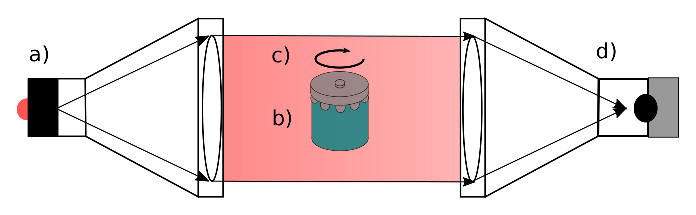
\includegraphics[width=10cm]{optical_ct.eps}
   \captionv{12}{Short title - optical CT scanner schematics}
   {Schematics of the optical CT scanner and dosimeter placement. The light 	source (a) consists of a small isotropic source (wavelength of 633 nm) 		and a Fresnel lens. The dosimeter is fixed to the scanner with a clamp 	(b), which secures one end of the dosimeter, and its rotated 360${}^{\circ}$ in small steps by a stepper motor. A CCD camera (d) images the light transmitted through the dosimeter for every rotation angle.
   \label{fig_example} 
    }  %note label inside caption
    \end{center}
\end{figure}

\begin{figure}[ht]
   \begin{center}
   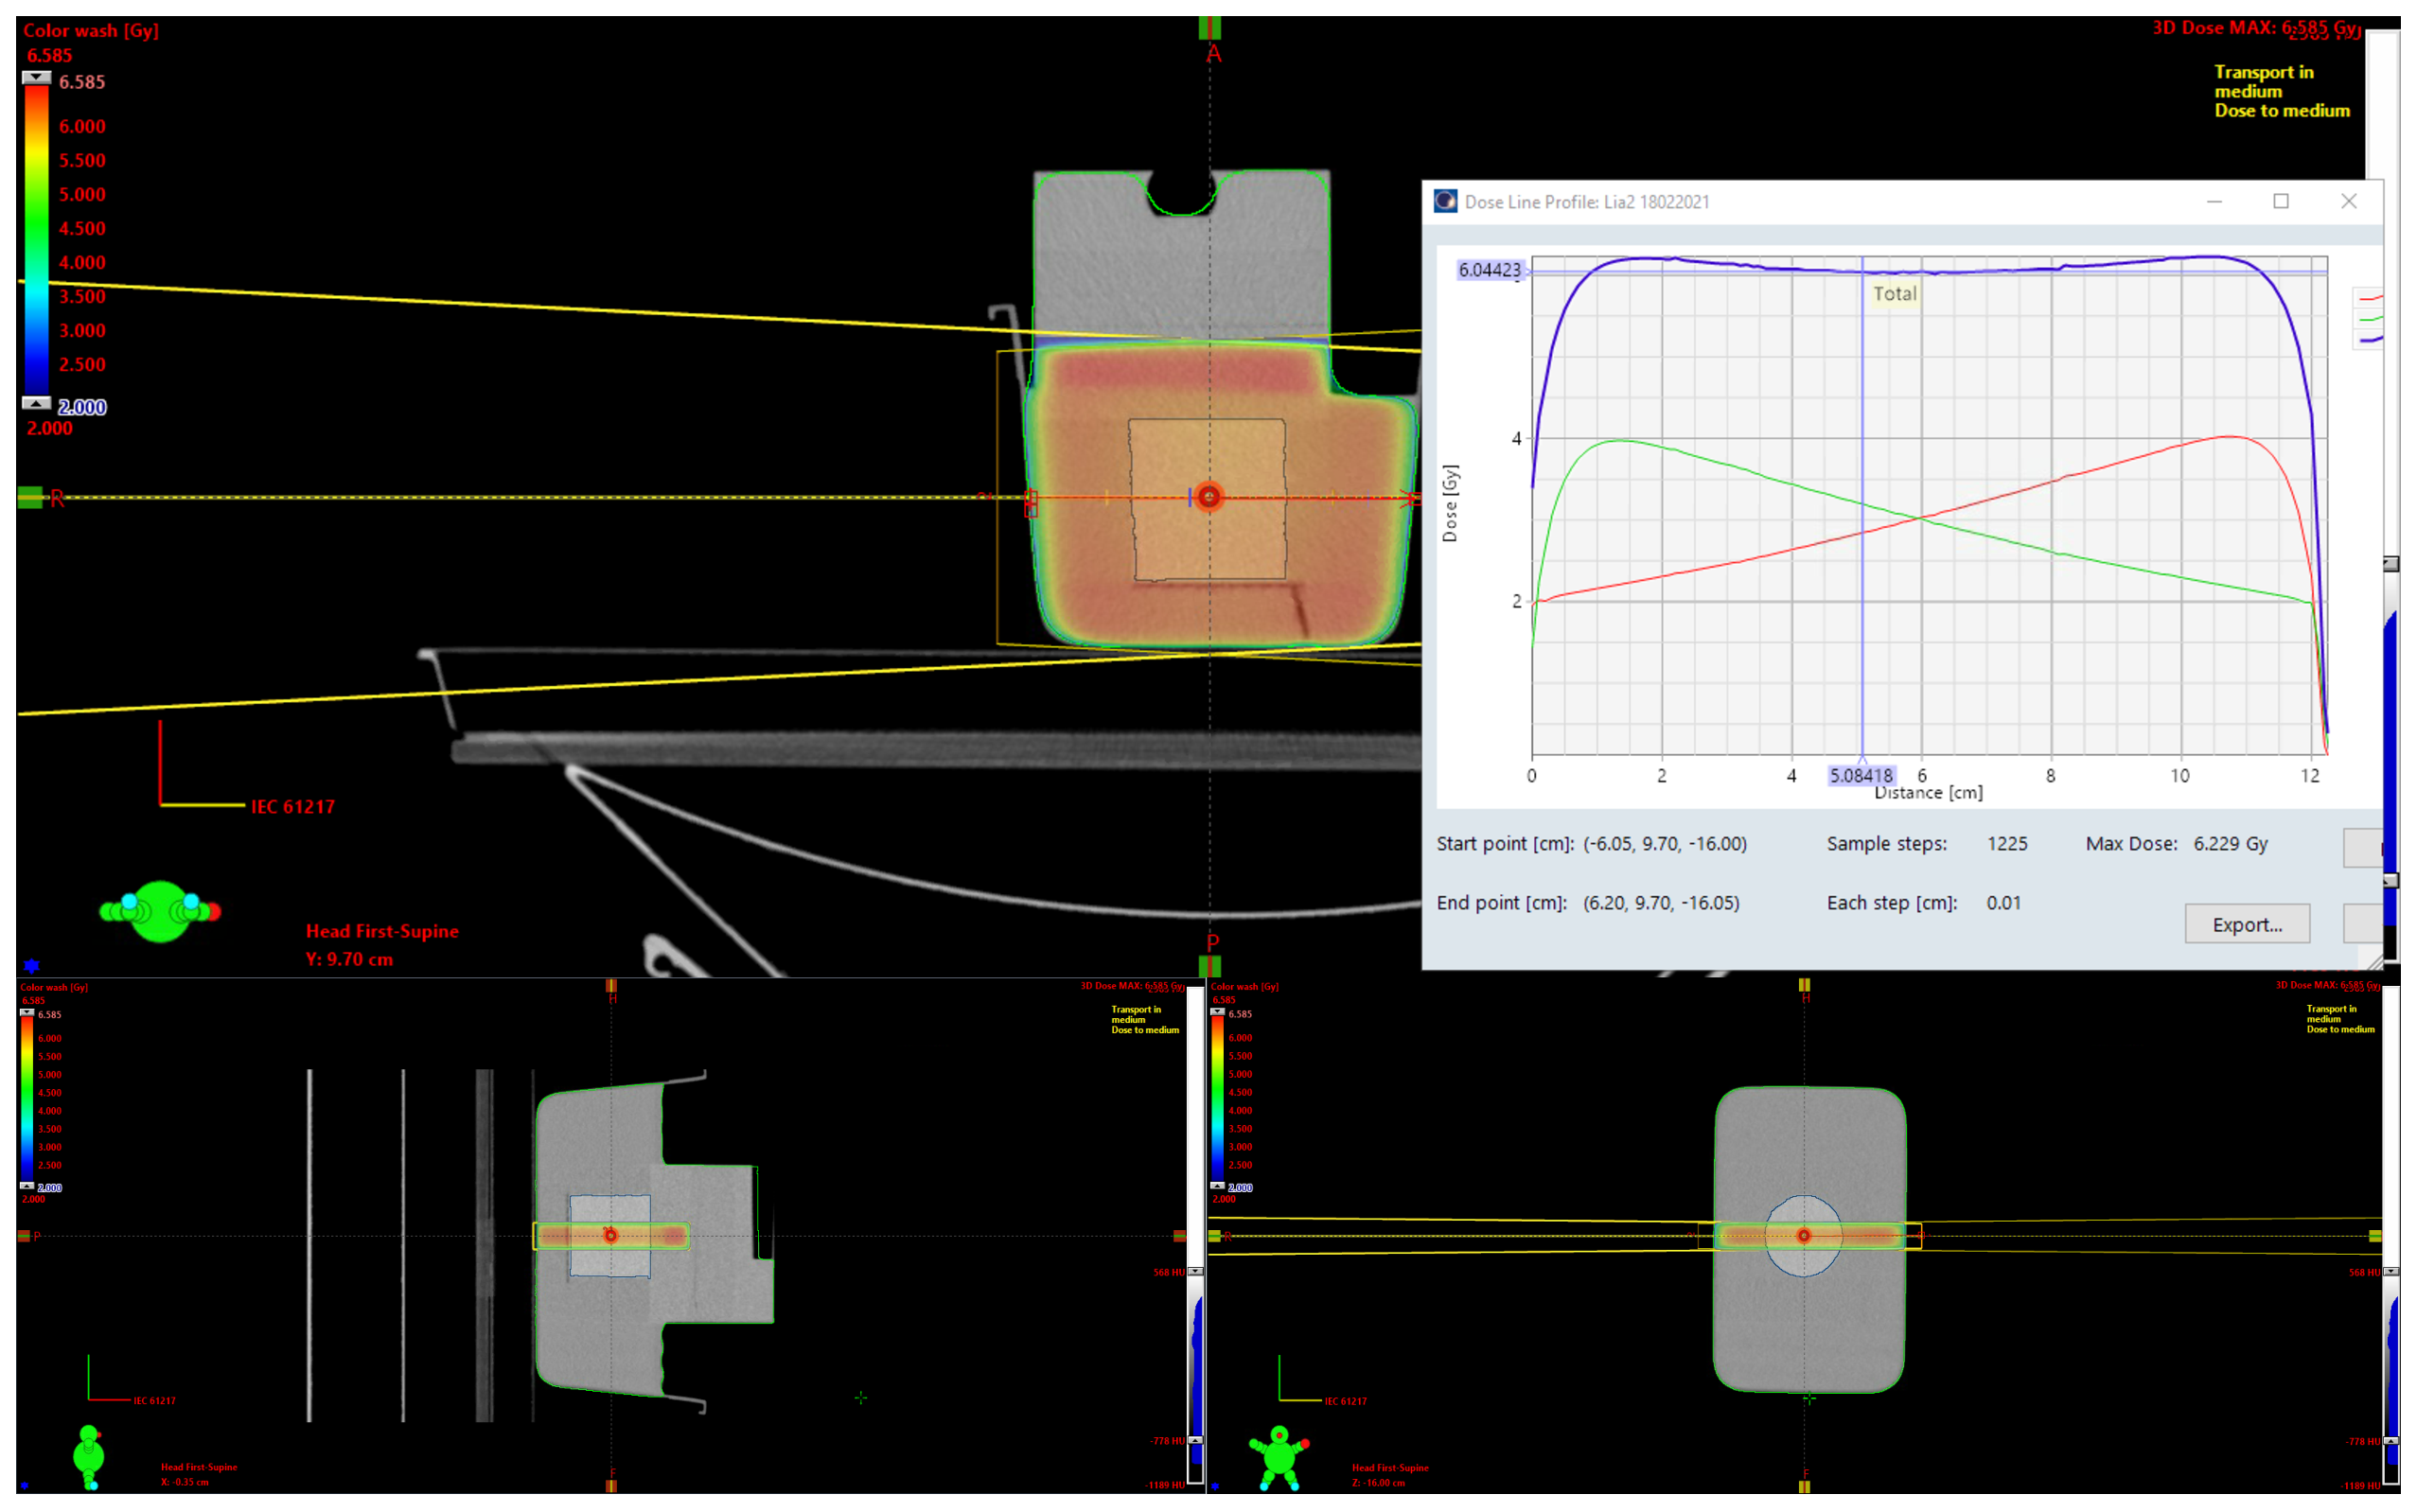
\includegraphics[width=15
cm]{TPS_images.eps}
   \captionv{12}{TPS plan}
   {TPS plan
   \label{fig_example1} 
    }  %note label inside caption
    \end{center}
\end{figure}

\clearpage


% following only if there is an appendix
\section*{Appendix}
\addcontentsline{toc}{section}{\numberline{}Appendix}
Appendix text goes here if needed.

\section*{References}
\addcontentsline{toc}{section}{\numberline{}References}
\vspace*{-20mm}

% Following assumes you are using bibtex. However, for submission to the
% journal you MUST explicitly INCLUDE THE REFERENCES IN THE TEX FILE. 
% In that case you need the following

% \begin{thebibliography}{10}
% insert the .bbl file generated by bibtex here
	%This will be a series of entries from your .bib file formatted
	%something like
	%\bibitem{Me09}
        %{I.~Meijsing, B.~W.~Raaymakers, A.~J.~E.~Raaijmakers \it et al.},
        %\newblock {Dosimetry for the MRI accelerator: the impact of a 
	%magnetic field on the response of a Farmer NE2571 ionization chamber},
        %\newblock Phys. Med. Biol. {\bf 54}, 2993 -- 3002 (2009).

% \end{thebibliography}

% The following is when using bibtex and picks up the example.bib file

%\bibliography{Explicit address of .bib file}
\bibliography{./example}      %example.bib is on the same directory
% above points to where we find the master reference list
% and also causes the bibliography to be printed

% When creating your bibliography you should run bibtex on your local
% computer after running pdflatex on your .tex file. bibtex will
% generate a .bbl file.
% Copy the contents of this .bbl file into your main latex document,
% replacing the "\bibliography" command which was pointing at your .bib file.


% following defines style of .bbl file 

%\bibliographystyle{explicit relative path to medphy.bst}
\bibliographystyle{./medphy.bst}    %if this is installed on your system,
				    %it is not essential to have the    ./

% Note that you need to typeset once, then run bibtex, then typeset another
% two times to get the references working properly.


\end{document}
